\section{Graph Based Problem Formulation}
This section formulates the charge problem as a graph. The first subsection describes the intuition behind this graph-based approach and the second represents the graph as a series of equality and inequality constraints in a Mixed Integer Linear Program (MILP).  
\subsection{Graph Formulation}
A solution to the bus charge problem must reveal both \textit{when} and \textit{to which} bus a charger should connect, suggesting a model with two dimensions. The first dimension characterizes time and is given discretely in a left to right fashion. The second dimension encodes the charger state and extends vertically as shown in figure \ref{fig:graphGridStructure}.  The charger may occupy one of several states.  It may be connected to one of the $N$ buses, or it may be unconnected, giving a total of $N + 1$ charge states. The 2-D representation is encoded as a grid and a node, $n_{i,j}$, can be placed wherever a charge state and time index intersect. These nodes are used to represent a charger in the $i^{\text{th}}$ charge state during the $j^{\text{th}}$ time index (see figure \ref{fig:graphGridStructure}). For example, $n_{1,0}$ from figure \ref{fig:graphGridStructure} represents a state where a charger is connected to Bus 1 at $t_0$. 
\par However, the presence of nodes at every state-time intersection suggests that buses can always connect.  This does not reflect reality because buses cannot connect when they are away from the station. Nodes are therefore only present in the grid when a corresponding bus can connnect to a charger and are absent when a bus leaves the station. Consider the two bus scenario from figure \ref{fig:graphGridStructure} where buses 1 and 2 provide transit services at $t_0$, $t_3$, and $t_6$. The schedule is encoded by removing $n_{1,0}$, $n_{2,0}$, $n_{1,3}$,  $n_{2,3}$, $n_{1,6}$, and $n_{2,6}$ to reflect the grid shown in figure \ref{fig:busAvailComparison}. 
\begin{figure}
\centering
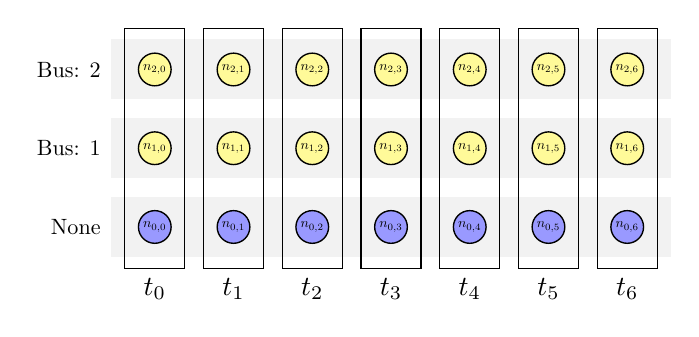
\begin{tikzpicture}
	\node[rectangle, fill=gray!10, minimum width=2.8in, minimum height=.3in,label=left:\scalebox{0.8}{Bus: 2}](bus2Box) at (3,1){};
	\node[rectangle, fill=gray!10, minimum width=2.8in, minimum height=.3in,label=left:\scalebox{0.8}{Bus: 1}](bus1Box) at (3,0){};
	\node[rectangle, fill=gray!10, minimum width=2.8in, minimum height=.3in,label=left:\scalebox{0.8}{None}](bus1Box) at (3,-1){};

	\node[circle, fill=yellow!40, line width=0.5pt, draw=black, minimum size=0.15in, inner sep=1pt](one) at (0,0){\scalebox{0.5}{$n_{1,0}$}};
	\node[circle, fill=yellow!40, line width=0.5pt, draw=black, minimum size=0.15in, inner sep=1pt](two) at (1,0){\scalebox{0.5}{$n_{1,1}$}}; 
	\node[circle, fill=yellow!40, line width=0.5pt, draw=black, minimum size=0.15in, inner sep=1pt](three) at (2,0){\scalebox{0.5}{$n_{1,2}$}};
	\node[circle, fill=yellow!40, line width=0.5pt, draw=black, minimum size=0.15in, inner sep=1pt](four) at (3,0){\scalebox{0.5}{$n_{1,3}$}};
	\node[circle, fill=yellow!40, line width=0.5pt, draw=black, minimum size=0.15in, inner sep=1pt](five) at (4,0){\scalebox{0.5}{$n_{1,4}$}};
	\node[circle, fill=yellow!40, line width=0.5pt, draw=black, minimum size=0.15in, inner sep=1pt](six) at (5,0){\scalebox{0.5}{$n_{1,5}$}};
	\node[circle, fill=yellow!40, line width=0.5pt, draw=black, minimum size=0.15in, inner sep=1pt](seven) at (6,0){\scalebox{0.5}{$n_{1,6}$}};

	\node[circle, fill=yellow!40, line width=0.5pt, draw=black, minimum size=0.15in, inner sep=1pt](eight) at (0,1){\scalebox{0.5}{$n_{2,0}$}};
	\node[circle, fill=yellow!40, line width=0.5pt, draw=black, minimum size=0.15in, inner sep=1pt](nine) at (1,1){\scalebox{0.5}{$n_{2,1}$}}; 
	\node[circle, fill=yellow!40, line width=0.5pt, draw=black, minimum size=0.15in, inner sep=1pt](ten) at (2,1){\scalebox{0.5}{$n_{2,2}$}};
	\node[circle, fill=yellow!40, line width=0.5pt, draw=black, minimum size=0.15in, inner sep=1pt](eleven) at (3,1){\scalebox{0.5}{$n_{2,3}$}};
	\node[circle, fill=yellow!40, line width=0.5pt, draw=black, minimum size=0.15in, inner sep=1pt](twelve) at (4,1){\scalebox{0.5}{$n_{2,4}$}};
	\node[circle, fill=yellow!40, line width=0.5pt, draw=black, minimum size=0.15in, inner sep=1pt](thirteen) at (5,1){\scalebox{0.5}{$n_{2,5}$}};
	\node[circle, fill=yellow!40, line width=0.5pt, draw=black, minimum size=0.15in, inner sep=1pt](fourteen) at (6,1){\scalebox{0.5}{$n_{2,6}$}};

	\node[circle, fill=blue!40, line width=0.5pt, draw=black, minimum size=0.15in, inner sep=1pt](eight) at (0,-1){\scalebox{0.5}{$n_{0,0}$}};
	\node[circle, fill=blue!40, line width=0.5pt, draw=black, minimum size=0.15in, inner sep=1pt](nine) at (1,-1){\scalebox{0.5}{$n_{0,1}$}}; 
	\node[circle, fill=blue!40, line width=0.5pt, draw=black, minimum size=0.15in, inner sep=1pt](ten) at (2,-1){\scalebox{0.5}{$n_{0,2}$}};
	\node[circle, fill=blue!40, line width=0.5pt, draw=black, minimum size=0.15in, inner sep=1pt](eleven) at (3,-1){\scalebox{0.5}{$n_{0,3}$}};
	\node[circle, fill=blue!40, line width=0.5pt, draw=black, minimum size=0.15in, inner sep=1pt](twelve) at (4,-1){\scalebox{0.5}{$n_{0,4}$}};
	\node[circle, fill=blue!40, line width=0.5pt, draw=black, minimum size=0.15in, inner sep=1pt](thirteen) at (5,-1){\scalebox{0.5}{$n_{0,5}$}};
	\node[circle, fill=blue!40, line width=0.5pt, draw=black, minimum size=0.15in, inner sep=1pt](fourteen) at (6,-1){\scalebox{0.5}{$n_{0,6}$}};

	\node[rectangle, draw, minimum width=0.3in, minimum height=1.2in,label=below:$t_0$](time0Box) at (0,0){};
	\node[rectangle, draw, minimum width=0.3in, minimum height=1.2in,label=below:$t_1$](time1Box) at (1,0){};
	\node[rectangle, draw, minimum width=0.3in, minimum height=1.2in,label=below:$t_2$](time2Box) at (2,0){};
	\node[rectangle, draw, minimum width=0.3in, minimum height=1.2in,label=below:$t_3$](time3Box) at (3,0){};
	\node[rectangle, draw, minimum width=0.3in, minimum height=1.2in,label=below:$t_4$](time4Box) at (4,0){};
	\node[rectangle, draw, minimum width=0.3in, minimum height=1.2in,label=below:$t_5$](time5Box) at (5,0){};
	\node[rectangle, draw, minimum width=0.3in, minimum height=1.2in,label=below:$t_6$](time6Box) at (6,0){}; 
\end{tikzpicture}
	\caption{Graph showing buses and timesteps}
	\label{fig:graphGridStructure} 
\end{figure}
\begin{figure}
\centering
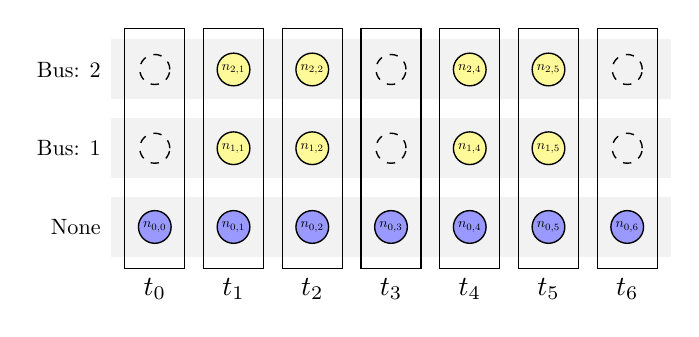
\begin{tikzpicture} 
	\node[rectangle, fill=gray!10, minimum width=2.8in, minimum height=.3in,label=left:\scalebox{0.8}{Bus: 2}](bus2Box) at (3,1){};
	\node[rectangle, fill=gray!10, minimum width=2.8in, minimum height=.3in,label=left:\scalebox{0.8}{Bus: 1}](bus1Box) at (3,0){};
	\node[rectangle, fill=gray!10, minimum width=2.8in, minimum height=.3in,label=left:\scalebox{0.8}{None}](bus1Box) at (3,-1){};

	\node[circle, draw, dashed,   line width=0.5pt, draw=black, minimum size=0.15in, inner sep=1pt](one)   at (0,0){};
	\node[circle, fill=yellow!40, line width=0.5pt, draw=black, minimum size=0.15in, inner sep=1pt](two)   at (1,0){\scalebox{0.5}{$n_{1,1}$}}; 
	\node[circle, fill=yellow!40, line width=0.5pt, draw=black, minimum size=0.15in, inner sep=1pt](three) at (2,0){\scalebox{0.5}{$n_{1,2}$}};
	\node[circle, draw, dashed,   line width=0.5pt, draw=black, minimum size=0.15in, inner sep=1pt](four)  at (3,0){};
	\node[circle, fill=yellow!40, line width=0.5pt, draw=black, minimum size=0.15in, inner sep=1pt](five)  at (4,0){\scalebox{0.5}{$n_{1,4}$}};
	\node[circle, fill=yellow!40, line width=0.5pt, draw=black, minimum size=0.15in, inner sep=1pt](six)   at (5,0){\scalebox{0.5}{$n_{1,5}$}};
	\node[circle, draw, dashed,   line width=0.5pt, draw=black, minimum size=0.15in, inner sep=1pt](seven) at (6,0){};

	\node[circle, draw, dashed,   line width=0.5pt, draw=black, minimum size=0.15in, inner sep=1pt](eight)    at (0,1){};
	\node[circle, fill=yellow!40, line width=0.5pt, draw=black, minimum size=0.15in, inner sep=1pt](nine)     at (1,1){\scalebox{0.5}{$n_{2,1}$}}; 
	\node[circle, fill=yellow!40, line width=0.5pt, draw=black, minimum size=0.15in, inner sep=1pt](ten)      at (2,1){\scalebox{0.5}{$n_{2,2}$}};
	\node[circle, draw, dashed,   line width=0.5pt, draw=black, minimum size=0.15in, inner sep=1pt](eleven)   at (3,1){};
	\node[circle, fill=yellow!40, line width=0.5pt, draw=black, minimum size=0.15in, inner sep=1pt](twelve)   at (4,1){\scalebox{0.5}{$n_{2,4}$}};
	\node[circle, fill=yellow!40, line width=0.5pt, draw=black, minimum size=0.15in, inner sep=1pt](thirteen) at (5,1){\scalebox{0.5}{$n_{2,5}$}};
	\node[circle, draw, dashed,   line width=0.5pt, draw=black, minimum size=0.15in, inner sep=1pt](fourteen) at (6,1){};

	\node[circle, fill=blue!40,   line width=0.5pt, draw=black, minimum size=0.15in, inner sep=1pt](eight)    at (0,-1){\scalebox{0.5}{$n_{0,0}$}};
	\node[circle, fill=blue!40,   line width=0.5pt, draw=black, minimum size=0.15in, inner sep=1pt](nine)     at (1,-1){\scalebox{0.5}{$n_{0,1}$}}; 
	\node[circle, fill=blue!40,   line width=0.5pt, draw=black, minimum size=0.15in, inner sep=1pt](ten)      at (2,-1){\scalebox{0.5}{$n_{0,2}$}};
	\node[circle, fill=blue!40,   line width=0.5pt, draw=black, minimum size=0.15in, inner sep=1pt](eleven)   at (3,-1){\scalebox{0.5}{$n_{0,3}$}};
	\node[circle, fill=blue!40,   line width=0.5pt, draw=black, minimum size=0.15in, inner sep=1pt](twelve)   at (4,-1){\scalebox{0.5}{$n_{0,4}$}};
	\node[circle, fill=blue!40,   line width=0.5pt, draw=black, minimum size=0.15in, inner sep=1pt](thirteen) at (5,-1){\scalebox{0.5}{$n_{0,5}$}};
	\node[circle, fill=blue!40,   line width=0.5pt, draw=black, minimum size=0.15in, inner sep=1pt](fourteen) at (6,-1){\scalebox{0.5}{$n_{0,6}$}};

	\node[rectangle, draw, minimum width=0.3in, minimum height=1.2in,label=below:$t_0$](time0Box) at (0,0){};
	\node[rectangle, draw, minimum width=0.3in, minimum height=1.2in,label=below:$t_1$](time1Box) at (1,0){};
	\node[rectangle, draw, minimum width=0.3in, minimum height=1.2in,label=below:$t_2$](time2Box) at (2,0){};
	\node[rectangle, draw, minimum width=0.3in, minimum height=1.2in,label=below:$t_3$](time3Box) at (3,0){};
	\node[rectangle, draw, minimum width=0.3in, minimum height=1.2in,label=below:$t_4$](time4Box) at (4,0){};
	\node[rectangle, draw, minimum width=0.3in, minimum height=1.2in,label=below:$t_5$](time5Box) at (5,0){};
	\node[rectangle, draw, minimum width=0.3in, minimum height=1.2in,label=below:$t_6$](time6Box) at (6,0){}; 
\end{tikzpicture}
	\caption{Bus availability represented in a graph}
	\label{fig:busAvailComparison}
\end{figure}

\par The state of a charger at any time is represented by occupying a corresponding node. Changes in charger state and time, are therefore reflected by a transition from one node to the next. These transitions are called edges (see figure \ref{fig:edgeNodeRel}) and represent decisions to connect to, charge, not charge, or disconnect from buses. An edge's decision is determined by the nodes on either end. Consider the edge from $n_{0,0}$ to $n_{0,1}$ in figure \ref{fig:edgeTypes}. This edge represents a no-charge decision because the nodes on both ends represent a disconnected charge state. Chargers cannot charge while disconnected, so the edge decision is no-charge.  Similarly, the edge between $n_{1,1}$ and $n_{1,2}$ indicates a to-charge decision as both $n_{1,1}$ and $n_{1,2}$ represent states where a charger is connected. Both to-charge and no-charge decisions are represented by \textit{horizontal} transitions in the graph and only reflect the passing of time as no changes to the physical hardware are made.
\par Conversely, diagonal transitions imply physical hardware changes because they represent decisions where chargers connect to or disconnect from a bus. One such example from figure \ref{fig:edgeTypes} includes the edge from $n_{0,0}$ to $n_{1,1}$. The state represented by $n_{0,0}$ is disconnected This edge represents an interval where a charger is disconnected at $t_0$ and connected at $t_1$, implying a `to-connect' decision. The same logic applies in reverse for the edge between $n_{1,2}$ and $n_{0,3}$. Hence, the bus charge problem can be described in terms of nodes and edges where nodes represent bus availability and edges encode all possible charge decisions. 
\par A charge schedule can be thought of as a list of charge decisions that govern charge behavior. Because decisions are represented by edges in the graph, a schedule is also represented by a sequence of connected edges that form a path through the graph. If an edge is selected, or active, it is considered part of the path.  Active and inactive edges are respectively represented edge weights equal to $1$, and $0$.
\par A graph with binary edge weights can only represent a plan for one charger. This representation can be expanded to represent an arbitrary number of chargers by using integer valued weights, where each weight gives the number of chargers in the transition.
\begin{figure}
	\centering
	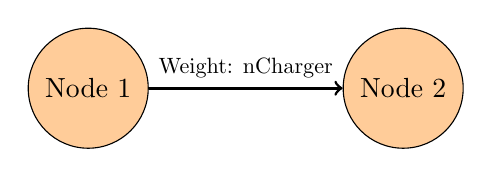
\begin{tikzpicture}
		\node[circle, draw, fill=orange!40, minimum size=0.6in](node1) at (0,0){Node 1};
		\node[circle, draw, fill=orange!40, minimum size=0.6in](node2) at (4,0){Node 2};
		\draw [->, line width=1pt] (node1.east) -- node[above]{\scalebox{0.8}{Weight: nCharger}}(node2.west); 
	\end{tikzpicture}
	\caption{Node to Node Connection}
	\label{fig:edgeNodeRel}
\end{figure} 
\begin{figure}
	\centering
	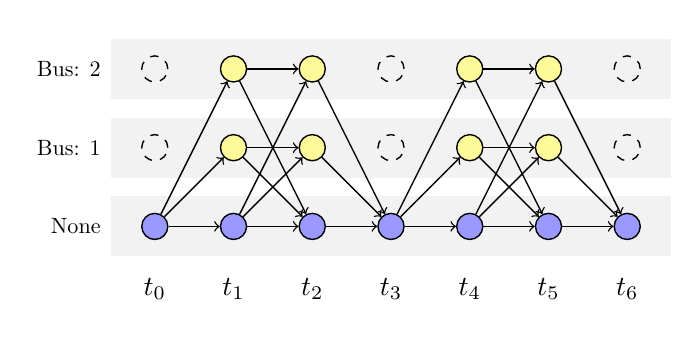
\begin{tikzpicture} 
		\node[rectangle, fill=gray!10, minimum width=2.8in, minimum height=.3in,label=left:\scalebox{0.8}{Bus: 2}](bus2Box) at (3,1){};
		\node[rectangle, fill=gray!10, minimum width=2.8in, minimum height=.3in,label=left:\scalebox{0.8}{Bus: 1}](bus1Box) at (3,0){};
		\node[rectangle, fill=gray!10, minimum width=2.8in, minimum height=.3in,label=left:\scalebox{0.8}{None}](bus1Box) at (3,-1){};

		\node[circle, draw, dashed, line width=0.5pt, draw=black, minimum size=0.1in](one) at (0,0){};
		\node[circle, fill=yellow!40, line width=0.5pt, draw=black, minimum size=0.1in](two) at (1,0){}; 
		\node[circle, fill=yellow!40, line width=0.5pt, draw=black, minimum size=0.1in](three) at (2,0){};
		\node[circle, draw, dashed, line width=0.5pt, draw=black, minimum size=0.1in](four) at (3,0){};
		\node[circle, fill=yellow!40, line width=0.5pt, draw=black, minimum size=0.1in](five) at (4,0){};
		\node[circle, fill=yellow!40, line width=0.5pt, draw=black, minimum size=0.1in](six) at (5,0){};
		\node[circle, draw, dashed,  line width=0.5pt, draw=black, minimum size=0.1in](seven) at (6,0){};

		\node[circle, draw, dashed, line width=0.5pt, draw=black, minimum size=0.1in](eight) at (0,1){};
		\node[circle, fill=yellow!40, line width=0.5pt, draw=black, minimum size=0.1in](nine) at (1,1){}; 
		\node[circle, fill=yellow!40, line width=0.5pt, draw=black, minimum size=0.1in](ten) at (2,1){};
		\node[circle, draw, dashed, line width=0.5pt, draw=black, minimum size=0.1in](eleven) at (3,1){};
		\node[circle, fill=yellow!40, line width=0.5pt, draw=black, minimum size=0.1in](twelve) at (4,1){};
		\node[circle, fill=yellow!40, line width=0.5pt, draw=black, minimum size=0.1in](thirteen) at (5,1){};
		\node[circle, draw, dashed, line width=0.5pt, draw=black, minimum size=0.1in](fourteen) at (6,1){};

		\node[circle, fill=blue!40, line width=0.5pt, draw=black, minimum size=0.1in](bOne) at (0,-1){};
		\node[circle, fill=blue!40, line width=0.5pt, draw=black, minimum size=0.1in](bTwo) at (1,-1){}; 
		\node[circle, fill=blue!40, line width=0.5pt, draw=black, minimum size=0.1in](bThree) at (2,-1){};
		\node[circle, fill=blue!40, line width=0.5pt, draw=black, minimum size=0.1in](bFour) at (3,-1){};
		\node[circle, fill=blue!40, line width=0.5pt, draw=black, minimum size=0.1in](bFive) at (4,-1){};
		\node[circle, fill=blue!40, line width=0.5pt, draw=black, minimum size=0.1in](bSix) at (5,-1){};
		\node[circle, fill=blue!40, line width=0.5pt, draw=black, minimum size=0.1in](bSeven) at (6,-1){};

		\node[rectangle, minimum width=0.3in, minimum height=1.2in,label=below:$t_0$](time0Box) at (0,0){};
		\node[rectangle, minimum width=0.3in, minimum height=1.2in,label=below:$t_1$](time1Box) at (1,0){};
		\node[rectangle, minimum width=0.3in, minimum height=1.2in,label=below:$t_2$](time2Box) at (2,0){};
		\node[rectangle, minimum width=0.3in, minimum height=1.2in,label=below:$t_3$](time3Box) at (3,0){};
		\node[rectangle, minimum width=0.3in, minimum height=1.2in,label=below:$t_4$](time4Box) at (4,0){};
		\node[rectangle, minimum width=0.3in, minimum height=1.2in,label=below:$t_5$](time5Box) at (5,0){};
		\node[rectangle, minimum width=0.3in, minimum height=1.2in,label=below:$t_6$](time6Box) at (6,0){}; 
		
		% draw rest edges
		\draw[->, line width=0.5pt] (bOne) -- (bTwo);
		\draw[->, line width=0.5pt] (bTwo) -- (bThree);
		\draw[->, line width=0.5pt] (bThree) -- (bFour);
		\draw[->, line width=0.5pt] (bFour) -- (bFive);
		\draw[->, line width=0.5pt] (bFive) -- (bSix);
		\draw[->, line width=0.5pt] (bSix) -- (bSeven);
		
		% draw connect edges
		\draw[->, line width=0.5pt] (bOne) -- (two); 
		\draw[->, line width=0.5pt] (bTwo) -- (three);
		\draw[->, line width=0.5pt] (bFour) -- (five);
		\draw[->, line width=0.5pt] (bFive) -- (six);

		\draw[->, line width=0.5pt] (bOne) -- (nine);
		\draw[->, line width=0.5pt] (bTwo) -- (ten);
		\draw[->, line width=0.5pt] (bFour) -- (twelve);
		\draw[->, line width=0.5pt] (bFive) -- (thirteen);

		% draw disconnect edges
		\draw[->, line width=0.5pt] (two) -- (bThree); 
		\draw[->, line width=0.5pt] (three) -- (bFour);
		\draw[->, line width=0.5pt] (five) -- (bSix);
		\draw[->, line width=0.5pt] (six) -- (bSeven);

		\draw[->, line width=0.5pt] (nine) -- (bThree);
		\draw[->, line width=0.5pt] (ten) -- (bFour);
		\draw[->, line width=0.5pt] (twelve) -- (bSix);
		\draw[->, line width=0.5pt] (thirteen) -- (bSeven);

		% draw charge edges
		\draw[->, line width=0.5pt] (two) -- (three);
		\draw[->, line width=0.5pt] (five) -- (six);
		\draw[->, line width=0.5pt] (nine) -- (ten);
		\draw[->, line width=0.5pt] (twelve) -- (thirteen);

	\end{tikzpicture}
	\caption{Graph-based model of the complete decision-space}
	\label{fig:completeGraph}
\end{figure}
\begin{figure}
	\centering
	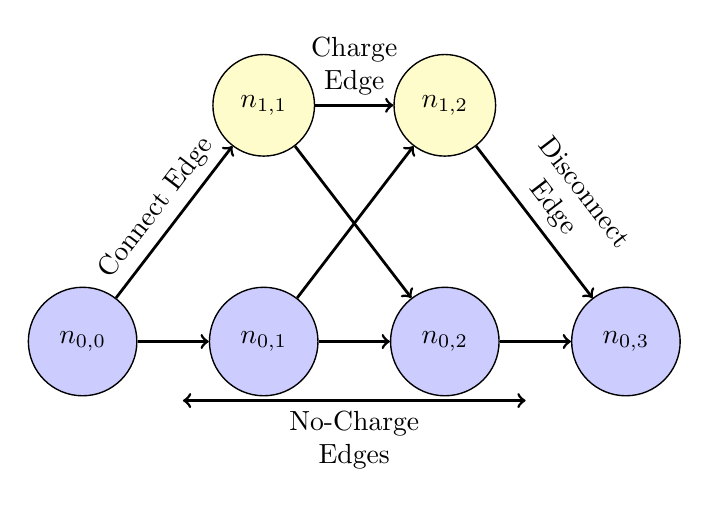
\begin{tikzpicture}
		\node[circle, fill=blue!20,line width=0.5pt, draw=black, text width=0.5in, inner sep=1pt,   align=center](one)   at (0,0)  {$n_{0,0}$};
		\node[circle, fill=blue!20,line width=0.5pt, draw=black, text width=0.5in, inner sep=1pt,   align=center](two)   at (2.3,0){$n_{0,1}$};
		\node[circle, fill=blue!20,line width=0.5pt, draw=black, text width=0.5in, inner sep=1pt,   align=center](three) at (4.6,0){$n_{0,2}$};
		\node[circle, fill=blue!20,line width=0.5pt, draw=black, text width=0.5in, inner sep=1pt,   align=center](four)  at (6.9,0){$n_{0,3}$};
		\node[circle, fill=yellow!20,line width=0.5pt, draw=black, text width=0.5in, inner sep=0in, align=center](five)  at (2.3,3){$n_{1,1}$};
		\node[circle, fill=yellow!20,line width=0.5pt, draw=black, text width=0.5in, inner sep=0in, align=center](six)   at (4.6,3){$n_{1,2}$};
		\node(placeholder1) at (1.15,-0.75){};
		\node(placeholder2) at (5.75,-0.75){};
		\draw [->, line width=1pt] (one) -- node[sloped, anchor=center, above, text width=2.5cm, midway, align=center]{Connect Edge}(five);
		\draw [->, line width=1pt] (one) -- (two);
		\draw [->, line width=1pt] (five) -- node[sloped, anchor=center, above, text width=1.5cm, midway, align=center]{Charge Edge}(six);
		\draw [->, line width=1pt] (five) -- (three);
		\draw [->, line width=1pt] (two) -- (six);
		\draw [->, line width=1pt] (six) -- node[sloped, anchor=center, above, text width=1.5cm, midway, align=center]{Disconnect Edge}(four);
		\draw [->, line width=1pt] (two) -- (three);
		\draw [->, line width=1pt] (three) -- (four); 
		\draw [<->, line width=1pt] (placeholder1) -- node[below, text width=2cm, midway, align=center]{No-Charge Edges}(placeholder2);
	\end{tikzpicture}
	\caption{Connect, Disconnect, and Charge Edges}
	\label{fig:edgeTypes}
\end{figure} 
\par Consider a three-charger scenario using the graph in figure \ref{fig:completeGraph}. A solution where one charger is connected to Bus 1 from $t_1$ to $t_2$ and to Bus 2 from $t_4$ to $t_5$ would be expressed by assigning unit weights to the appropriate connect, charge, and disconnect edges.  The second charger remains idle as illustrated by the active edges along the bottom row of charger states (see figure \ref{fig:graphWithSolution}).  
\par In summary, the graph encodes bus availability with nodes, decisions with edges, and schedules with edge weights. Solving the bus charge problem becomes a matter of finding the optimal set of edge weights, where optimal is used to denote the most cost effective charge plan.

\begin{figure}
	\centering
	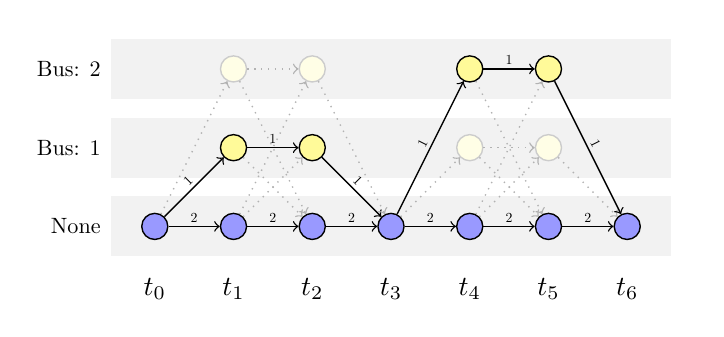
\begin{tikzpicture} 
		\node[rectangle, fill=gray!10, minimum width=2.8in, minimum height=.3in,label=left:\scalebox{0.8}{Bus: 2}](bus2Box) at (3,1){};
		\node[rectangle, fill=gray!10, minimum width=2.8in, minimum height=.3in,label=left:\scalebox{0.8}{Bus: 1}](bus1Box) at (3,0){};
		\node[rectangle, fill=gray!10, minimum width=2.8in, minimum height=.3in,label=left:\scalebox{0.8}{None}](bus1Box) at (3,-1){};

		\node[circle, fill=yellow!40, line width=0.5pt, draw=black, minimum size=0.1in](two) at (1,0){}; 
		\node[circle, fill=yellow!40, line width=0.5pt, draw=black, minimum size=0.1in](three) at (2,0){};
		\node[circle, fill=yellow!10, line width=0.5pt, draw=black!20, minimum size=0.1in](five) at (4,0){};
		\node[circle, fill=yellow!10, line width=0.5pt, draw=black!20, minimum size=0.1in](six) at (5,0){};

		\node[circle, fill=yellow!10, line width=0.5pt, draw=black!20, minimum size=0.1in](nine) at (1,1){}; 
		\node[circle, fill=yellow!10, line width=0.5pt, draw=black!20, minimum size=0.1in](ten) at (2,1){};
		\node[circle, fill=yellow!40, line width=0.5pt, draw=black, minimum size=0.1in](twelve) at (4,1){};
		\node[circle, fill=yellow!40, line width=0.5pt, draw=black, minimum size=0.1in](thirteen) at (5,1){};

		\node[circle, fill=blue!40, line width=0.5pt, draw=black, minimum size=0.1in](bOne) at (0,-1){};
		\node[circle, fill=blue!40, line width=0.5pt, draw=black, minimum size=0.1in](bTwo) at (1,-1){}; 
		\node[circle, fill=blue!40, line width=0.5pt, draw=black, minimum size=0.1in](bThree) at (2,-1){};
		\node[circle, fill=blue!40, line width=0.5pt, draw=black, minimum size=0.1in](bFour) at (3,-1){};
		\node[circle, fill=blue!40, line width=0.5pt, draw=black, minimum size=0.1in](bFive) at (4,-1){};
		\node[circle, fill=blue!40, line width=0.5pt, draw=black, minimum size=0.1in](bSix) at (5,-1){};
		\node[circle, fill=blue!40, line width=0.5pt, draw=black, minimum size=0.1in](bSeven) at (6,-1){};

		\node[rectangle, minimum width=0.3in, minimum height=1.2in,label=below:$t_0$](time0Box) at (0,0){};
		\node[rectangle, minimum width=0.3in, minimum height=1.2in,label=below:$t_1$](time1Box) at (1,0){};
		\node[rectangle, minimum width=0.3in, minimum height=1.2in,label=below:$t_2$](time2Box) at (2,0){};
		\node[rectangle, minimum width=0.3in, minimum height=1.2in,label=below:$t_3$](time3Box) at (3,0){};
		\node[rectangle, minimum width=0.3in, minimum height=1.2in,label=below:$t_4$](time4Box) at (4,0){};
		\node[rectangle, minimum width=0.3in, minimum height=1.2in,label=below:$t_5$](time5Box) at (5,0){};
		\node[rectangle, minimum width=0.3in, minimum height=1.2in,label=below:$t_6$](time6Box) at (6,0){}; 
		
		% draw rest edges
		\draw[->, line width=0.5pt] (bOne) -- node [text width=2.5cm, midway, above=-2.1pt, align=center]{\scalebox{0.5}{2}}(bTwo);
		\draw[->, line width=0.5pt] (bTwo) -- node [text width=2.5cm, midway, above=-2.1pt, align=center]{\scalebox{0.5}{2}}(bThree);
		\draw[->, line width=0.5pt] (bThree) -- node [text width=2.5cm, midway, above=-2.1pt, align=center]{\scalebox{0.5}{2}}(bFour);
		\draw[->, line width=0.5pt] (bFour) -- node [text width=2.5cm, midway, above=-2.1pt, align=center]{\scalebox{0.5}{2}}(bFive);
		\draw[->, line width=0.5pt] (bFive) -- node [text width=2.5cm, midway, above=-2.1pt, align=center]{\scalebox{0.5}{2}}(bSix);
		\draw[->, line width=0.5pt] (bSix) -- node [text width=2.5cm, midway, above=-2.1pt, align=center]{\scalebox{0.5}{2}}(bSeven);
		
		% draw connect edges
		\draw[->, line width=0.5pt] (bOne) -- node [sloped, text width=2.5cm, midway, above=-2.1pt, align=center]{\scalebox{0.5}{1}}(two); 
		\draw[->, dotted, color=black!30, line width=0.5pt] (bTwo) -- (three);
		\draw[->, dotted, color=black!30, line width=0.5pt] (bFour) -- (five);
		\draw[->, dotted, color=black!30, line width=0.5pt] (bFive) -- (six);

		\draw[->, dotted, color=black!30, line width=0.5pt] (bOne) -- (nine);
		\draw[->, dotted, color=black!30, line width=0.5pt] (bTwo) -- (ten);
		\draw[->, line width=0.5pt] (bFour) -- node [sloped, text width=2.5cm, midway, above=-2.1pt, align=center]{\scalebox{0.5}{1}}(twelve);
		\draw[->, dotted, color=black!30, line width=0.5pt] (bFive) -- (thirteen);

		% draw disconnect edges
		\draw[->, dotted, color=black!30, line width=0.5pt] (two) -- (bThree); 
		\draw[->, line width=0.5pt] (three) -- node [sloped, text width=2.5cm, midway, above=-2.1pt, align=center]{\scalebox{0.5}{1}}(bFour);
		\draw[->, dotted, color=black!30, line width=0.5pt] (five) -- (bSix);
		\draw[->, dotted, color=black!30, line width=0.5pt] (six) -- (bSeven);

		\draw[->, dotted, color=black!30, line width=0.5pt] (nine) -- (bThree);
		\draw[->, dotted, color=black!30, line width=0.5pt] (ten) -- (bFour);
		\draw[->, dotted, color=black!30, line width=0.5pt] (twelve) -- (bSix);
		\draw[->, line width=0.5pt] (thirteen) -- node [sloped, text width=2.5cm, midway, above=-2.1pt, align=center]{\scalebox{0.5}{1}}(bSeven);

		% draw charge edges
		\draw[->, line width=0.5pt] (two) -- node [text width=2.5cm, midway, above=-2.1pt, align=center]{\scalebox{0.5}{1}}(three);
		\draw[->, dotted, color=black!30, line width=0.5pt] (five) -- (six);
		\draw[->, dotted, color=black!30, line width=0.5pt] (nine) -- (ten);
		\draw[->, line width=0.5pt] (twelve) -- node [text width=2.5cm, midway, above=-2.1pt, align=center]{\scalebox{0.5}{1}}(thirteen); 
	\end{tikzpicture}
	\caption{One solution to a 2-bus 3-charger scenario}
	\label{fig:graphWithSolution}
\end{figure}

\subsection{Graph Constraints}
\par Finding the optimal charge schedule can be expressed as an optimization problem, where the graph is encoded through equality/inequality constraints for a Mixed Integer Linear Program of the form 
\begin{equation}
	\begin{aligned}
		& \underset{\mathbf{y}}{\text{min}}\ \mathbf{r}^T\mathbf{y} \ \text{subject to} \\
		& F\mathbf{y} = \mathbf{f}, \ Q\mathbf{y} \le \mathbf{q}
	\end{aligned},
\end{equation}
where the equality and inequality constraints are encoded in $F$, $\mathbf{f}$, $Q$ and $\mathbf{q}$. The variable $\mathbf{y}$ is a vector containing the elements of the solution and is of the form 
\begin{equation}\label{eqn:y}
		\mathbf{y} = \begin{bmatrix}
		\mathbf{x} \\
		\mathbf{d} \\
		\mathbf{g} \\
		\mathbf{e} \\
		\mathbf{p} \\
		\hat{p} \\
		\hat{p}_\text{off-peak} \\
		\hat{p}_\text{on-peak} 
	\end{bmatrix},
\end{equation}
where each element of $\mathbf{y}$ is defined later in this paper.
\par  This subsection formulates two sets of constraints.  The first encodes the graph, enforces conservation of chargers, and defines the number of chargers through a set of net-flow constraints. The second prevents the charger from reconnecting shortly after disconnecting, and allows only a single charger to connect at a time by enforcing group-flow constraints.
\subsubsection{\label{sec:net-flow} Net-Flow Constraints}
\begin{align}\label{eqn:flow}
	A\mathbf{x}=\mathbf{c}_f,	
\end{align}
where $A$ is the graph incidence matrix, $\mathbf{x}$ is the $\text{nEdge} \times 1$ vector of edge weights and corresponds to $\mathbf{x}$ in equation \ref{eqn:y}, and $\mathbf{c}_f$ is $\text{nNode} \times 1$ and equals the difference between incoming and outgoing edge weights, or \textit{net-flow}.
\par  An incidence matrix organizes relationships between nodes and edges by describing which edges leave and enter which nodes. The matrix $A$ is an nNode $\times$ nEdge matrix and expresses incoming connections between the $i^{\text{th}}$ node and $j^{\text{th}}$ edge as $A_{i,j} = 1$. Similarly, outgoing connections are given with $A_{i,j} = -1$, and no connection with $A_{i,j} = 0$. For example, the graph in figure \ref{fig:genericGraph} is represented as:
\begin{figure}
	\centering
	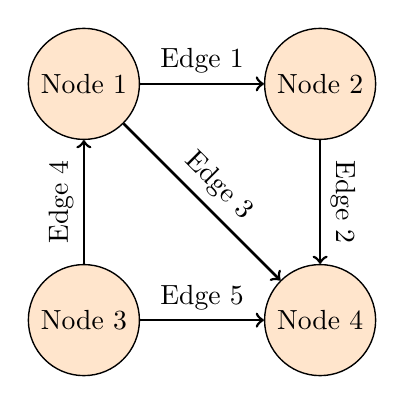
\begin{tikzpicture}
		\node[circle, line width=0.5pt, draw=black, fill=orange!20, minimum size=0.5in](topLeft) at (0,3){Node 1};
		\node[circle, line width=0.5pt, draw=black, fill=orange!20, minimum size=0.5in](topRight) at (3,3){Node 2};
		\node[circle, line width=0.5pt, draw=black, fill=orange!20, minimum size=0.5in](btmLeft) at (0,0){Node 3};
		\node[circle, line width=0.5pt, draw=black, fill=orange!20, minimum size=0.5in](btmRight) at (3,0){Node 4};
		\draw [->, line width=1pt] (topLeft.east) -- node [text width=2.5cm, midway, above, align=center]{Edge 1}(topRight.west);
		\draw [->, line width=1pt] (btmLeft.north) -- node [sloped, anchor=center, above, text width=2.5cm, midway, align=center]{Edge 4}(topLeft.south);
		\draw [->, line width=1pt] (topLeft.south east) -- node [sloped, anchor=center, above, text width=2.5cm, midway, align=center]{Edge 3}(btmRight.north west);
		\draw [->, line width=1pt] (topRight.south) -- node[sloped, anchor=center, above, text width=2.5cm, midway, align=center]{Edge 2}(btmRight.north);
		\draw [->, line width=1pt] (btmLeft.east) -- node[text width=2.5cm, midway, above, align=center]{Edge 5}(btmRight.west);
	\end{tikzpicture}
	\caption{A generic directed graph consisting of nodes and edges}
	\label{fig:genericGraph}
\end{figure}
\begin{align}
	\begin{bmatrix}
		-1 & 0 & -1 & 1 & 0 \\
		1 & -1 & 0 & 0 & 0 \\
		0 & 0 & 0 & -1 & -1 \\
		0 & 1 & 1 & 0 & 1 \\
	\end{bmatrix}
\end{align}
\par  The difference between the number of chargers entering and leaving, or the \textit{net-flow}, can be expressed in terms of $A$ as seen in equation \ref{eqn:flow}.  Because the number of chargers must be conserved, the number of incoming and outgoing chargers must be equal. This is expressed in linear form as $a_i^{T}x = 0$, where $a_i$ is the $i^{\text{th}}$ row of $A$. The only exceptions occur at \textit{source} and \textit{sink} nodes.
\par A source node represents the beginning state for all chargers.  Because edges originate here, there are no incoming edges and the net-flow will be minus the number of chargers. This is described in linear form as $a_i^Tx = -\text{nCharger}$.
\par Sink nodes represent the final state, where all edges terminate (see figure \ref{fig:sourceSink}). Because sinks have no outgoing edges, they maintain a positive net-flow equal to the number of chargers and is expressed as $a_i^T = \text{nCharger}$. 
\par Therefore, the \textit{flow constraints} require that $c_f$ be equal to zero for all non-source and non-sink nodes as seen in equation \ref{eqn:cFlow}.  
\begin{figure}
	\centering
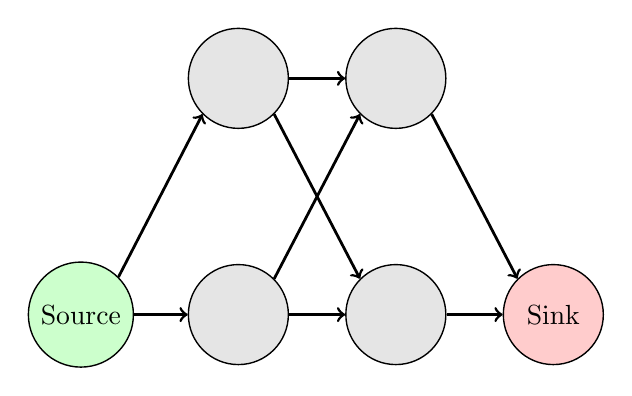
\begin{tikzpicture}
	\node[circle, fill=green!20, line width=0.5pt, draw=black, minimum size=0.5in](one) at (0,0){Source};
	\node[circle, fill=gray!20,line width=0.5pt, draw=black, minimum size=0.5in](two) at (2,0){};
	\node[circle, fill=gray!20,line width=0.5pt, draw=black, minimum size=0.5in](three) at (4,0){};
	\node[circle, fill=red!20,line width=0.5pt, draw=black, minimum size=0.5in](four) at (6,0){Sink};
	\node[circle, fill=gray!20, line width=0.5pt, draw=black, minimum size=0.5in](five) at (2,3){};
	\node[circle, fill=gray!20, line width=0.5pt, draw=black, minimum size=0.5in](six) at (4,3){};
	\draw [->, line width=1pt] (one.north east) -- (five.south west);
	\draw [->, line width=1pt] (one.east) -- (two.west);
	\draw [->, line width=1pt] (five.east) -- (six.west);
	\draw [->, line width=1pt] (five.south east) -- (three.north west);
	\draw [->, line width=1pt] (two.north east) -- (six.south west);
	\draw [->, line width=1pt] (six.south east) -- (four.north west);
	\draw [->, line width=1pt] (two.east) -- (three.west);
	\draw [->, line width=1pt] (three.east) -- (four.west); 
\end{tikzpicture}
	\caption{Network flow illustrating sources and sinks}
	\label{fig:sourceSink} 
\end{figure} 
\begin{align}\label{eqn:cFlow}
	Ax = \begin{bmatrix} 0 \\ \vdots \\ -\text{nCharger} \\ \vdots \\ 0 \\ \text{nCharger} \\ \vdots \\ 0\end{bmatrix}.
\end{align}
Equation \ref{eqn:cFlow} can be formulated in terms of $\mathbf{y}$ by appropriatly zero-padding $A$ such that
\begin{equation}\label{eqn:cFlow2}
	\begin{aligned}
		c_f &= \begin{bmatrix}A & 0 \end{bmatrix}\mathbf{y}\\
		    &= \tilde{A} \mathbf{y} 
	\end{aligned}
\end{equation}
\subsubsection{Group-flow Constraints}
\par Another flow type, known as group flow, can be used to regulate the number of chargers entering a set of nodes. This is desired for two reasons:  It avoids multiple reconnects during a charge period, and limits the number of connecting chargers to one. 
\par Define a charge group as the set of all nodes for a given bus corresponding to one station visit as shown in figure \ref{fig:groups}. The \textit{group flow} is the number of chargers that enter a group and is represented as the sum of all incoming edge weights (see figure \ref{fig:groupedEdges}). 
\par Denote the $\text{nGroup} \times \text{nEdge}$ group incidence matrix as $B$, where $B_{i,j}$ is $1$ if the $j^{\text{th}}$ edge enters the $i^{\text{th}}$ group and $0$ otherwise. For example, the group incidence matrix corresponding to the graph in figure \ref{fig:groupEdges} contains $1$ in the $7^{\text{th}}$ and $10^{\text{th}}$ columns for Group 1, and the $12^{\text{th}}$ and $15^{\text{th}}$ columns for group 2 as given in equation \ref{eqn:groupB}.
\begin{align}\label{eqn:groupB}
	B = \begin{bmatrix}0 \; 0 \; 0 \; 0 \; 0 \; 0 \; 1 \; 0 \; 0 \; 1 \; 0 \; 0 \; 0 \; 0 \; 0 \; 0\\
	                   0 \; 0 \; 0 \; 0 \; 0 \; 0 \; 0 \; 0 \; 0 \; 0 \; 0 \; 1 \; 0 \; 0 \; 1 \; 0\end{bmatrix}
\end{align}

\begin{figure}
	\centering
	\begin{tikzpicture}
		\node[circle, fill=blue!20, line width=0.5pt, draw=black, minimum size=0.1in](one) at (0,0){};
		\node[circle, fill=blue!20, line width=0.5pt, draw=black, minimum size=0.1in](two) at (1,0){}; 
		\node[circle, fill=blue!20, line width=0.5pt, draw=black, minimum size=0.1in](three) at (2,0){};
		\node[circle, fill=blue!20, line width=0.5pt, draw=black, minimum size=0.1in](four) at (3,0){};
		\node[circle, fill=blue!20, line width=0.5pt, draw=black, minimum size=0.1in](five) at (4,0){};
		\node[circle, fill=blue!20, line width=0.5pt, draw=black, minimum size=0.1in](six) at (5,0){};
		\node[circle, fill=blue!20, line width=0.5pt, draw=black, minimum size=0.1in](seven) at (6,0){};
		\node[circle, fill=yellow!20, line width=0.5pt, draw=black, minimum size=0.1in](eight) at (1,2){};
		\node[circle, fill=yellow!20, line width=0.5pt, draw=black, minimum size=0.1in](nine) at (2,2){};
		\node[circle, fill=yellow!20, line width=0.5pt, draw=black, minimum size=0.1in](ten) at (4,2){}; 
		\node[circle, fill=yellow!20, line width=0.5pt, draw=black, minimum size=0.1in](eleven) at (5,2){}; 
		\draw [->, line width=0.5pt] (one.east) -- (two.west);
		\draw [->, line width=0.5pt] (two.east) -- (three.west);
		\draw [->, line width=0.5pt] (three.east) -- (four.west);
		\draw [->, line width=0.5pt] (four.east) -- (five.west);
		\draw [->, line width=0.5pt] (five.east) -- (six.west);
		\draw [->, line width=0.5pt] (six.east) -- (seven.west);
		\draw [->, line width=0.5pt] (one.north east) -- (eight.south west);
		\draw [->, line width=0.5pt] (two.north east) -- (nine.south west);
		\draw [->, line width=0.5pt] (four.north east) -- (ten.south west);
		\draw [->, line width=0.5pt] (five.north east) -- (eleven.south west);
		\draw [->, line width=0.5pt] (eight.south east) -- (three.north west);
		\draw [->, line width=0.5pt] (nine.south east) -- (four.north west);
		\draw [->, line width=0.5pt] (ten.south east) -- (six.north west);
		\draw [->, line width=0.5pt] (eleven.south east) -- (seven.north west);
		\draw [->, line width=0.5pt] (eight.east) -- (nine.west);
		\draw [->, line width=0.5pt] (ten.east) -- (eleven.west); 
		\node[ellipse, fill opacity=0.2, draw opacity=0.5, line width=0.5pt, draw=orange!40,fill=orange!40, minimum height=0.4in, minimum width=1in, label=Group 1](group1) at (1.5,2){};
		\node[ellipse, fill opacity=0.2, draw opacity=0.5, line width=0.5pt, draw=purple!40,fill=purple!40,  minimum height=0.4in, minimum width=1in, label=Group 2](group2) at (4.5,2){};
	\end{tikzpicture}
	\caption{Example of groups in a network flow graph}
	\label{fig:groups}
\end{figure}
\begin{figure}
\centering
	\begin{tikzpicture}
		\node[circle, fill=blue!20, line width=0.5pt, draw=black, minimum size=0.1in](one) at (0,0){};
		\node[circle, fill=blue!20, line width=0.5pt, draw=black, minimum size=0.1in](two) at (1,0){}; 
		\node[circle, fill=blue!20, line width=0.5pt, draw=black, minimum size=0.1in](three) at (2,0){};
		\node[circle, fill=blue!20, line width=0.5pt, draw=black, minimum size=0.1in](four) at (3,0){};
		\node[circle, fill=blue!20, line width=0.5pt, draw=black, minimum size=0.1in](five) at (4,0){};
		\node[circle, fill=blue!20, line width=0.5pt, draw=black, minimum size=0.1in](six) at (5,0){};
		\node[circle, fill=blue!20, line width=0.5pt, draw=black, minimum size=0.1in](seven) at (6,0){};
		\node[circle, fill=yellow!20, line width=0.5pt, draw=black, minimum size=0.1in](eight) at (1,2){};
		\node[circle, fill=yellow!20, line width=0.5pt, draw=black, minimum size=0.1in](nine) at (2,2){};
		\node[circle, fill=yellow!20, line width=0.5pt, draw=black, minimum size=0.1in](ten) at (4,2){}; 
		\node[circle, fill=yellow!20, line width=0.5pt, draw=black, minimum size=0.1in](eleven) at (5,2){}; 
		\draw [->, line width=0.5pt,color=black!40] (one.east) -- (two.west);
		\draw [->, line width=0.5pt,color=black!40] (two.east) -- (three.west);
		\draw [->, line width=0.5pt,color=black!40] (three.east) -- (four.west);
		\draw [->, line width=0.5pt,color=black!40] (four.east) -- (five.west);
		\draw [->, line width=0.5pt,color=black!40] (five.east) -- (six.west);
		\draw [->, line width=0.5pt,color=black!40] (six.east) -- (seven.west);
		\draw [->, color=orange, line width=0.75pt] (one.north east) -- (eight.south west);
		\draw [->, color=orange, line width=0.75pt] (two.north east) -- (nine.south west);
		\draw [->, color=purple, line width=0.75pt] (four.north east) -- (ten.south west);
		\draw [->, color=purple, line width=0.75pt] (five.north east) -- (eleven.south west);
		\draw [->, line width=0.5pt,color=black!40] (eight.south east) -- (three.north west);
		\draw [->, line width=0.5pt,color=black!40] (nine.south east) -- (four.north west);
		\draw [->, line width=0.5pt,color=black!40] (ten.south east) -- (six.north west);
		\draw [->, line width=0.5pt,color=black!40] (eleven.south east) -- (seven.north west);
		\draw [->, line width=0.5pt,color=black!40] (eight.east) -- (nine.west);
		\draw [->, line width=0.5pt,color=black!40] (ten.east) -- (eleven.west); 
		\node[ellipse, line width=0pt, draw opacity=0.5, fill opacity=0.2, fill=purple!40, draw=purple!40, minimum height=0.4in, minimum width=1in, label=Group 2](group2) at (4.5,2){};
		\node[ellipse, line width=0pt, draw opacity=0.5, fill opacity=0.2, fill=orange!40, draw=orange!40, minimum height=0.4in, minimum width=1in, label=Group 1](group1) at (1.5,2){};
	\end{tikzpicture}
	\caption{Incoming Group Edges}
	\label{fig:groupedEdges} 
\end{figure} 
Let $\mathbf{x}$ be the edge weights as before and $\mathbf{c}_g$ be an nGroup $\times$ 1 vector where the $i^{\text{th}}$ element gives the group flow for group $i$. The group flow is then computed as 
\begin{align}\label{eqn:cGroupFlow}
	B\mathbf{x} = \mathbf{c}_g
\end{align}
But the group flow is required to be one at most to avoid thrashing.  This is expressed by the inequality given in equation \ref{eqn:cGroupFlow}.
\begin{align}\label{eqn:cGroupFlow}
	Bx \le \begin{bmatrix} 1\\ 1 \\\vdots \\ 1\end{bmatrix}.
\end{align}
Similarly to equation \ref{eqn:cFlow2}, equation \ref{eqn:cGroupFlow} can also be expressed in terms of $\mathbf{y}$ with appropriate zero padding as
\begin{equation}\label{eqn:cGroupFlow2}
	\begin{aligned}
		\begin{bmatrix} B & 0\end{bmatrix} \mathbf{y} &= \mathbf{1} \\
		\tilde{B}\mathbf{y} &= \mathbf{1}.
	\end{aligned}
\end{equation}
\subsection{Section Summary} In summary, the bus charge problem can be formulated as a graph with nodes and edges, where charge plans are encoded as a path. The charge problem aims to find a feasible path which minimizes the cost of power. Feasibility is defined through a set of net-flow and group-flow constraints. Net-flow constraints are encoded through an adjacency matrix and enforce both the conservation and total number of chargers. The group-flow constraints prevent charge thrashing and regulate the number of simultaneous charger-to-bus connections. 
\begin{figure}
\centering
	\begin{tikzpicture}
		\node[circle, fill=blue!20, line width=0.5pt, draw=black, minimum size=0.1in](one) at (0,0){};
		\node[circle, fill=blue!20, line width=0.5pt, draw=black, minimum size=0.1in](two) at (1,0){}; 
		\node[circle, fill=blue!20, line width=0.5pt, draw=black, minimum size=0.1in](three) at (2,0){};
		\node[circle, fill=blue!20, line width=0.5pt, draw=black, minimum size=0.1in](four) at (3,0){};
		\node[circle, fill=blue!20, line width=0.5pt, draw=black, minimum size=0.1in](five) at (4,0){};
		\node[circle, fill=blue!20, line width=0.5pt, draw=black, minimum size=0.1in](six) at (5,0){};
		\node[circle, fill=blue!20, line width=0.5pt, draw=black, minimum size=0.1in](seven) at (6,0){};
		\node[circle, fill=yellow!20, line width=0.5pt, draw=black, minimum size=0.1in](eight) at (1,2){};
		\node[circle, fill=yellow!20, line width=0.5pt, draw=black, minimum size=0.1in](nine) at (2,2){};
		\node[circle, fill=yellow!20, line width=0.5pt, draw=black, minimum size=0.1in](ten) at (4,2){}; 
		\node[circle, fill=yellow!20, line width=0.5pt, draw=black, minimum size=0.1in](eleven) at (5,2){}; 
		\node[ellipse, line width=0pt, draw opacity=0.5, fill opacity=0.2, fill=purple!40, draw=purple!40, minimum height=0.4in, minimum width=1in, label=Group 2](group2) at (4.5,2){};
		\node[ellipse, line width=0pt, draw opacity=0.5, fill opacity=0.2, fill=orange!40, draw=orange!40, minimum height=0.4in, minimum width=1in, label=Group 1](group1) at (1.5,2){};
		\draw [->, line width=0.5pt,color=black!40] (one.east) -- (two.west);
		\draw [->, line width=0.5pt,color=black!40] (two.east) -- (three.west);
		\draw [->, line width=0.5pt,color=black!40] (three.east) -- (four.west);
		\draw [->, line width=0.5pt,color=black!40] (four.east) -- (five.west);
		\draw [->, line width=0.5pt,color=black!40] (five.east) -- (six.west);
		\draw [->, line width=0.5pt,color=black!40] (six.east) -- (seven.west);
		\draw [->, color=orange, line width=0.75pt] (one.north east) -- node[sloped, anchor=center, above, text width=2.5cm, align=center]{Edge 7}(eight.south west);
		\draw [->, color=orange, line width=0.75pt] (two.north east) -- node[sloped, anchor=center, above, text width=2.5cm, align=center]{Edge 10}(nine.south west);
		\draw [->, color=purple, line width=0.75pt] (four.north east) -- node[sloped, anchor=center, above, text width=2.5cm, align=center]{Edge 12}(ten.south west);
		\draw [->, color=purple, line width=0.75pt] (five.north east) -- node[sloped, anchor=center, above, text width=2.5cm, align=center]{Edge 15}(eleven.south west);
		\draw [->, line width=0.5pt,color=black!40] (eight.south east) -- (three.north west);
		\draw [->, line width=0.5pt,color=black!40] (nine.south east) -- (four.north west);
		\draw [->, line width=0.5pt,color=black!40] (ten.south east) -- (six.north west);
		\draw [->, line width=0.5pt,color=black!40] (eleven.south east) -- (seven.north west);
		\draw [->, line width=0.5pt,color=black!40] (eight.east) -- (nine.west);
		\draw [->, line width=0.5pt,color=black!40] (ten.east) -- (eleven.west); 
	\end{tikzpicture}
	\caption{Connect edge example for groups}
	\label{fig:groupEdges} 
\end{figure} 
